% $Id: template.tex 11 2007-04-03 22:25:53Z jpeltier $

%\documentclass{vgtc}                          % final (conference style)
%\documentclass[review]{vgtc}                 % review
%\documentclass[widereview]{vgtc}             % wide-spaced review
%\documentclass[preprint]{vgtc}               % preprint
\documentclass[electronic]{vgtc}             % electronic version

%% Uncomment one of the lines above depending on where your paper is
%% in the conference process. ``review'' and ``widereview'' are for review
%% submission, ``preprint'' is for pre-publication, and the final version
%% doesn't use a specific qualifier. Further, ``electronic'' includes
%% hyperreferences for more convenient online viewing.

%% Please use one of the ``review'' options in combination with the
%% assigned online id (see below) ONLY if your paper uses a double blind
%% review process. Some conferences, like IEEE Vis and InfoVis, have NOT
%% in the past.

%% Figures should be in CMYK or Grey scale format, otherwise, colour 
%% shifting may occur during the printing process.

%% These few lines make a distinction between latex and pdflatex calls and they
%% bring in essential packages for graphics and font handling.
%% Note that due to the \DeclareGraphicsExtensions{} call it is no longer necessary
%% to provide the the path and extension of a graphics file:
%% \includegraphics{diamondrule} is completely sufficient.
%%
\ifpdf%                                % if we use pdflatex
  \pdfoutput=1\relax                   % create PDFs from pdfLaTeX
  \pdfcompresslevel=9                  % PDF Compression
  \pdfoptionpdfminorversion=7          % create PDF 1.7
  \ExecuteOptions{pdftex}
  \usepackage{graphicx}                % allow us to embed graphics files
  \DeclareGraphicsExtensions{.pdf,.png,.jpg,.jpeg} % for pdflatex we expect .pdf, .png, or .jpg files
\else%                                 % else we use pure latex
  \ExecuteOptions{dvips}
  \usepackage{graphicx}                % allow us to embed graphics files
  \DeclareGraphicsExtensions{.eps}     % for pure latex we expect eps files
\fi%

%% it is recomended to use ``\autoref{sec:bla}'' instead of ``Fig.~\ref{sec:bla}''
\graphicspath{{figures/}{pictures/}{images/}{./}} % where to search for the images

\usepackage{microtype}                 % use micro-typography (slightly more compact, better to read)
\PassOptionsToPackage{warn}{textcomp}  % to address font issues with \textrightarrow
\usepackage{textcomp}                  % use better special symbols
\usepackage{mathptmx}                  % use matching math font
\usepackage{times}                     % we use Times as the main font
\renewcommand*\ttdefault{txtt}         % a nicer typewriter font
\usepackage{cite}                      % needed to automatically sort the references
\usepackage{tabu}                      % only used for the table example
\usepackage{booktabs}                  % only used for the table example
%% We encourage the use of mathptmx for consistent usage of times font
%% throughout the proceedings. However, if you encounter conflicts
%% with other math-related packages, you may want to disable it.


%% If you are submitting a paper to a conference for review with a double
%% blind reviewing process, please replace the value ``0'' below with your
%% OnlineID. Otherwise, you may safely leave it at ``0''.
\onlineid{0}

%% declare the category of your paper, only shown in review mode
\vgtccategory{Summary}

%% allow for this line if you want the electronic option to work properly
\vgtcinsertpkg

%% In preprint mode you may define your own headline.
%\preprinttext{To appear in an IEEE VGTC sponsored conference.}

%% Paper title.

\title{Survey: Visual Analysis Approaches to Time Series Prediction}

%% This is how authors are specified in the conference style

%% Author and Affiliation (single author).
\author{Fabian Otto\thanks{e-mail: fabian.otto@stud.tu-darmstadt.de}}
\affiliation{\scriptsize Technische Universit\"at Darmstadt}

%% A teaser figure can be included as follows, but is not recommended since
%% the space is now taken up by a full width abstract.
%\teaser{
%  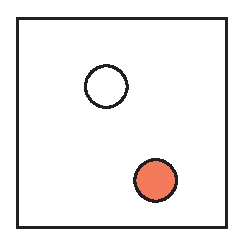
\includegraphics[width=1.5in]{sample.eps}
%  \caption{Lookit! Lookit!}
%}

%% Abstract section.
%\abstract{
%%	Do I need this one?\\
%	\textbf{General questions for Lena}:\\
%%	It seems to me I do not have enough sources. \\
%%	Couple more pictures missing esp. spatiotemporal\\
%	Are some systems too much into detail?\\
%	Due to missing space I reduced, the systems I found later on to just a couple of sentences.
%	Should I include more of those, because they sound more interesting? (this is completely subjective question for you).
%	For now, I thought including them is better than leaving them out.
%	It gives the reader at least some point to start from.\\
%	Not sure about the introduction, though.\\
%	Currently I do not see enough space to do this sort summary of important steps in time series analysis as you mention. I probably skip that, don't I?\\
%	Still, somehow it is hard to define any structure in the first part, the systems are so different. 
%	Maybe model and data driven?! But then again, almost all approaches are data driven and, I think, only one is not.
%	Another thing, which seams plausible is general models and application specific approaches. 
%	But the same problem here, besides time searcher they all tend to have a primary focus problem and try to generalize as good as possible.\\
%	PS: Without abstract, it is exactly 4 pages plus one page references
%} % end of abstract

% \nocopyrightspace

%%%%%%%%%%%%%%%%%%%%%%%%%%%%%%%%%%%%%%%%%%%%%%%%%%%%%%%%%%%%%%%%
%%%%%%%%%%%%%%%%%%%%%% START OF THE PAPER %%%%%%%%%%%%%%%%%%%%%%
%%%%%%%%%%%%%%%%%%%%%%%%%%%%%%%%%%%%%%%%%%%%%%%%%%%%%%%%%%%%%%%%%

\begin{document}

\firstsection{Introduction}

\maketitle

Making predictions about the future is a common problem in corporate scenarios as well as in everyones personal life. 
Corporations need predictions in order to determine e.g. the following day's demand on the market or which new product has the highest Return on Investment.
This is also true for the personal live, when buying a new laptop or signing a contract.
These decisions are easier if there is at least some certainty about future events.\\
According to Lu et al. \cite{Lu:2017} predictive analytics is concerned with the prediction of future outcomes and trends based past observations. 
It comprises an approach that includes pattern recognition, extrapolation and algorithmic modeling associated with domain knowledge.
Contrary to that, descriptive or prescriptive systems are reactive and provide information after the decision was made or populate decision models respectively.
Consequently, predictive analysis can be seen in between these two in the way of applying historical data to generate knowledge about the future.
%Predictive Visual Analytics typically relies on four different steps \cite{Lu:2017}:
%\begin{enumerate}
%	\item Data Preprocessing
%	\item Feature Engineering
%	\item Modeling
%	\item Result Exploration and Validation
%\end{enumerate}
Time series are often highly complex, depend on different variables and cannot be easily predicted. 
Common models to analyze time series are often based on the Box-Jenkins method \cite{box:2015} or on regression \cite{draper:2014}.
These automatic approaches provide analysts with forecasts.
However, they are often not able to provide analysts with an understanding of interesting phenomena.
This means analysts cannot easily include their domain knowledge in the modeling process in order to create better predictive models.
In combination with visual analytics, analysts have an interactive solution, which enables them to answer a wider range of research questions, such as: 
\begin{enumerate}
	\item[(Q1)] What are global trends within the time series?
	\item[(Q2)] Which local patterns, seasonal trends and important events/periods can be found?
	\item[(Q3)] Which model is the best to represent the time series?
	\item[(Q4)] How can this information be used to detect anomalies and turning points, which may change the future direction of the time series?
	\item[(Q5)] Which correlations between variables can be found?
	\item[(Q6)] Which parameters are influencing my production process?
	\item[(Q7)] How certain is my current prediction? 
\end{enumerate}
% interactively search for global trends (1) and local cyclic patterns (2), i.e. seasonal effects.
%This allows them to detect anomalies and turning points, which may change the future direction of the time series.
%Additionally, analysts can identify important events/periods of time, such as the weeks before Christmas.\\
This survey will mainly focus on questions (Q1) and (Q2) in \autoref{subsec:trend}, on (Q3) in \autoref{subsec:selection} and (Q4), (Q5), (Q6) in \autoref{subsec:correlation}.
(Q7) is addressed throughout all sections.
Nevertheless, time series prediction is an ambiguous field and some overlap might occur.\\
Moreover, in some cases additional information about the location are available and have to be included in the pattern detection and prediction process. 
In spatiotemporal analysis, analysts search for regions with unusually high occurrences of events, also called hotspots.
For cases where these hotspots are found, analysts would like to predict how these regions will develop and where new hotspots may occur in order to come up with better decisions.
Prominent applications areas involve: detecting outbreaks of diseases as well as crime and terror developments. \\
Hence, the goal is to provide the reader with an entry point to select an appropriate approach according to her/his currently required area of application. 

\section{Abstract Time Series\label{sec:temporal}}
Abstract time series only utilize the time dimension in order to predict future events or find patterns.
This includes 
%TODO

\subsection{Trend Detection\label{subsec:trend}}
The most common problem in time series prediction is trend detection.
This involves finding a overall global trend or a more specific local trend, e.g. seasonal changes in retail due to Christmas.
In regression analysis this can expressed as finding a predictive function 
\[
y(\textbf{x,w}) = \textbf{w}_0 + \sum_{j=0}^{M-1} \textbf{w}_j \phi_j(\textbf{x})
\]
where $M$ represents the models parameters and $\phi(\cdot)$ a feature function to model the desired behavior. 
Unfortunately, these kind of models hardly allow the analyst to include domain knowledge in the prediction process.\\

An older Visual Analytics approaches can be found from Ichikawa et al. \cite{ichikawa:2002}.
Their goal was to enable stock analysts to predict multiple daytime stock prices and simultaneously visualize a set of predictions from different simulation systems. 
This means their system mainly supports result exploration by efficiently visualizing a vast amount of predictions.
As a consequence, the visualization includes multiple predictions for multiple stocks. 
Further, one major finding was, visualizing multivariate predictions in a 3-dimensional space creates high levels of occlusion, thus, it is not suitable to provide an easy and intuitive way of visualization.
Instead, the system utilizes line charts with cluttering control and a color band display with level-of-detail control (\autoref{fig:color-band}). 

\begin{figure}[htb]
	\centering
	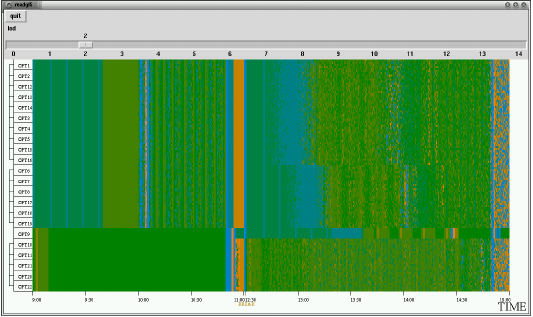
\includegraphics[width=\columnwidth]{color-band}
	\caption{Color band display \cite{ichikawa:2002}}
	\label{fig:color-band}
\end{figure}

The color band display reduces the complexity of the predictive time series as large amounts of simulations typically create occlusions within the line plot.
This issue can also be found in TimeSearcher \cite{buono:2007}, which displays the mean instead.
The color band is created by assigning similar predictions to the same cluster and consequently reducing the time series to a color band, i.e. its key elements and overall trend of each cluster.
Therefore, the analyst is able to detect discrepancies between the clusters and compare specific predictions with the overall trend. 
For additional comparison, the system's workspace visualizes a set of predictions for different parameter ranges (e.g. sales organizations) as well as different stocks.
Whereas the different parameter ranges could also support the analyst in answering (Q3).
Consequently, the user can detect trends concerning the whole stock market and answer (Q1).  
However, due to the amount of simulations displayed, it might be hard to extract specific information.
The color band display lowers the complexity significantly, hence this system is not able to answer (Q2) properly.
Additionally, the system is not visualizing any information about the simulations' certainty and makes it hard for an analyst to determine, which simulations are more important and fails to answer (Q7).

In contrast to Ichikawa et al.\cite{ichikawa:2002} the system of Hao et al. \cite{Hao:2011, Hao:2009} explicitly focuses on time series prediction with peak preservation and is able to provide the analyst with better answers to (Q2).
Identified peaks are explicitly included in the systems forecast.
In their work they focus on cell based power consumption data in data centers, for which it is especially important to have deeper knowledge of peaks.
They applied an automated peak preserving smoothing method in order to reduce noise and get a more reliable prediction as well as retain the seasonality of the data.
Thereby, the analyst is able to determine the influence of more recent measurements, i.e. how far back in time seasonality is considered in the smoothing process. 
Further, the system provides a visualization of its prediction quality on the historical time series, which allows the analyst to judge the quality of the current model (Q7). 
It has to be mentioned here, that including a peak preservation is sometimes not wanted.
For example when predicting the market's demand, the global trend is more important and including peaks may induce more uncertainty. 
A large drawback of those systems is their univariate focus, therefore they may be insufficient in a lot of practical applications.

Visualizing uncertainty was one of the analyst questions the system of Ichikawa et al. \cite{ichikawa:2002} was not able to answer.
A popular choice to address this problem is based on ensemble visualizations, which were only partially applied, however the visualization was restricted to the color band display and the analyst was not presented with the certainty based on multiple predictions. 
The system from K\"opp et al. \cite{koepp:2014} provides a heatmap-based option to visualize multiple time series predictions. 
Their interactive solution offers analysts an comprehensive analysis of the predictions certainties with e.g. quantiles, extrema and percentiles. 
%Further, similar to Ichikawa et al., the analyst is able to detect diverging trends within the given ensembles. 
Another resembling feature to Ichikawa et al. \cite{ichikawa:2002} is the external source of simulations. 
Depending on the application area, this can be beneficial or disadvantages. 
Analysts can used their existing ensemble and visualize it, but it is more complicated to begin with if no such analysis environment is present. 
Other ensemble approaches incorporate models explicitly and help in general to answer (Q7), but this is beyond the scope of the survey and the reader is encouraged to use this work as a entry point for further research. 

During the evaluation of TiMoVa \cite{boegl:2013}, (further details about this tool in \autoref{subsec:selection}) they found that an actual prediction functionality would provide additional value for the analyst during the model selection.
Therefore, B\"oegel et al. \cite{boegl:2014} included a result exploration and validation functionality.
This allows the analyst to adjust different model parameters and see real time changes in the corresponding prediction visualizations.
Consequently, the analyst gets feedback about the adequateness of the chosen model and can simultaneously use the provided visualizations after the selection process to search for trends to answer (Q1) and (Q2).
%Similar to \cite{buono:2007}, the prediction is incorporated with confidence bands to express the models certainty. 
The models certainty is incorporated with displaying confidence bands.
Additionally, they specifically visualize the difference of true and predicted values for each data point as well as the direction (positive or negative).
This gives the analyst a quick overview if the model is constantly over- or underestimating the time series as well as how long and often this occurs and is not provided by any of the other models.

\subsection{Model Selection\label{subsec:selection}}
Besides searching for trends with a visual analytics system directly, analyst are often interested in creating a model. 
Models have the advantage that they can be used by unexperienced users once they are defined as well as in automatic systems. 
However, as mentioned in the previous chapter simply applying a model is restricting the analyst. 
Therefore, model selection approaches want to support analysts in finding the best model for their forecast, so that domain knowledge can be included as much as possible. 
More precisely, during model selection the systems support the analyst with e.g. subspace exploration, training set modification, parameter tuning. \cite{Lu:2017}\\
A popular approach for general abstract time series analysis is from Buono et al. \cite{buono:2005}.
It focuses on automatically detecting similar patterns compared to a user specified pattern.
The system was built upon TimeSearcher proposed by Hochheiser and Shneiderman \cite{Hochheiser:2004}, which concentrates on high usability even for users without specialized skills such as in statistics.
%Based on their idea, Buono et al. continued with using timeboxes, i.e. rectangular regions that filter the data and reduce the scope of each search.
%Their updated version adds another variant for pattern search in the remaining data. 
%Further, they also allow users to work with long time series of multiple heterogeneous variables. 
However, these two version of TimeSearcher are more interested in data exploration and consequently would be located before the model selection step to provide the analyst with a better understanding of the data. 
%either in the data preprocessing or as supporting tool in the feature engineering step. 
%For data exploration the user is initially presented with a multivariable time series viewer, which allows to visually analyze multiple variables in parallel on different levels-of-detail.
%In order to detect reoccurring and similar patterns, the user highlights a found pattern within the time series and the system uses a similarity-based search to find other occurrences. 
%Therefor, the search space can be limited to only interesting areas.
%The initial matches of the given pattern can afterwards be refined to support the analysis goal better. 
%This process of returning many results and consequently enable the user to reduce the outcome to his/her liking, can also be found in spatiotemporal approaches (\autoref{sec:spatiotemp}), esp. in the template driven approach of \cite{malik:2014}.
%Moreover, TimeSearcher also provides different data transformations to match patterns more easily. 
%One drawback of the system is that it cannot deal with missing data points and pattern matching is very depended on the user's chosen parameters.
To assist the model selection process, the updated version of TimeSearcher by Buono et al. \cite{buono:2007} is providing additional features.  
These additional features include an actual prediction functionality and a preview interface with different parameter selection tools.
For the prediction, TimeSearcher resorts on the similarity-based approach, which was used in the previous version \cite{buono:2005} to detect time series with similar behavior.
In order to provide the analyst with an better overall understanding of the selected subset of time series, the system offers a summarized view based on a river plot, which also incorporates confidence bands (bottom right of \autoref{fig:timesearcher}) as in the following system TiMoVa \cite{boegl:2013} .
The actual prediction is computed by extrapolating only those time series, which were identified as similar to the target time series.
As in \cite{buono:2005} the system is meant for users without statistical knowledge.
In order enable the analyst to select a better model, the simultaneous preview interface allows to compare multiple parameter choices as well as different modeling techniques, such as smoothing, in parallel (\autoref{fig:timesearcher}).
This idea of displaying different parameter outcomes is also included in the stock price prediction from \cite{ichikawa:2002}.
Given the data-driven nature of the system, this requires the analyst to provide larger datasets compared to a model-driven approach.
Further, the actual prediction is only using the mean and thus might not be able to represent more complex data sets. 
However, the simultaneous preview interface simplifies the modeling process and makes it accessible to untrained users and allows experienced analysts to get a better insight.

\begin{figure}[htb]
	\centering
	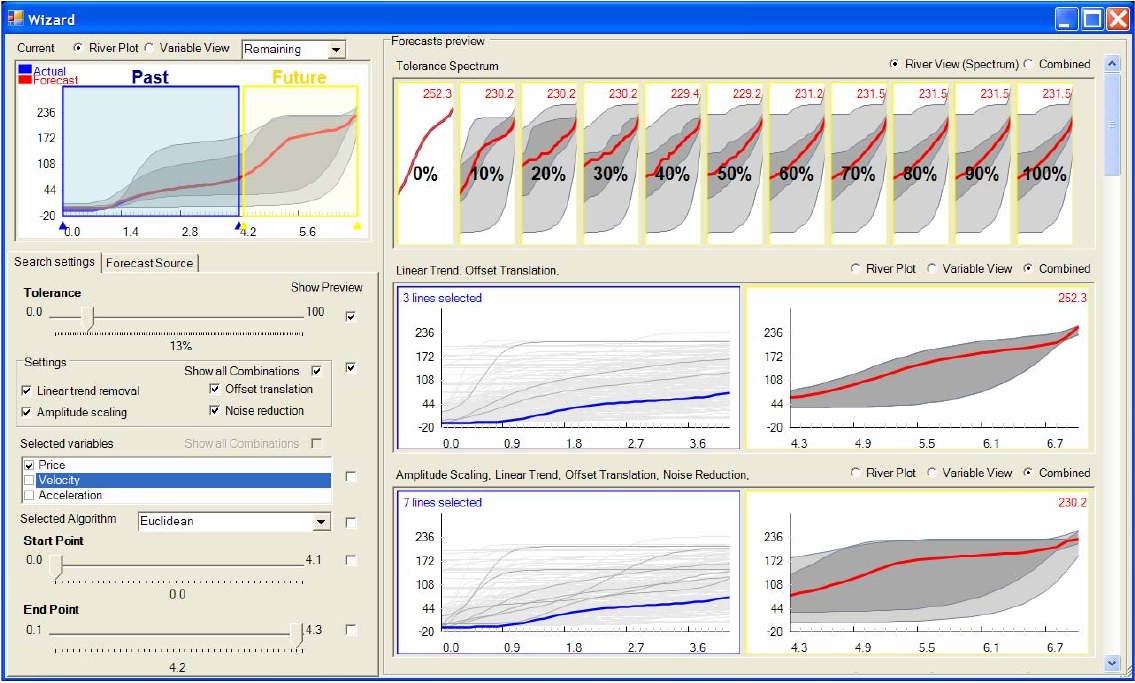
\includegraphics[width=\columnwidth]{TimeSearcher}
	\caption{TimeSearcher's \cite{buono:2007} simultaneous preview interface
	}
	\label{fig:timesearcher}
\end{figure}

In practical scenarios the requirement to have large amounts of data points can often be a problem, which makes all versions of TimeSearcher \cite{Hochheiser:2004, buono:2005, buono:2007} less valuable.
Consequently, a model-driven system, which requires less data points, is preferred.
The approach of Ichikawa et al. \cite{ichikawa:2002} could be seen as such system as it utilizes external simulations models.
However, it is not supporting the modeling process and is therefore only seen as system for trend detection.
On the other hand TiMoVa \cite{boegl:2013} explicitly provides a model selection tool for traditionally successful models such as ARIMA, AR, MA, etc.
As consequence, the system is designed after the Box-Jenkins method and is supporting the model specification and selection process.
For model specification, i.e. selection of an appropriate model type and its order, they provide autocorrelation function and partial autocorrelation function plots.
These plots are also utilized by the analyst to select the model's parameters.
Validation can be done, besides the interactive visualization of the prediction and its certainty, as described in \autoref{subsec:trend}, by different residual analysis plots and key figures.
A big drawback of the system are its assumptions about the preprocessed data. 
It requires a time series without missing values and only supports univariate analysis.

Apart from Box-Jenkins approaches, regression models are a common choice. 
Further, with a growing social media use use\footnote{https://www.statista.com/statistics/272014/global-social-networks-ranked-by-number-of-users/}, those platforms may contain highly relevant information for predictions. 
Based on this, Lu et al. \cite{lu:2014} proposed a model selection framework including mainly social media information. 
Their framework also offers other functionalities such as sentiment analysis, however, for this survey the focus is only on the time series prediction feature.
Similar to TimeSearcher \cite{Hochheiser:2004, buono:2005, buono:2007}, they focus on users without prior knowledge in analysis and statistics and enable the analyst to validate the model on similar instances. 
Analogous to TiMoVa's extension \cite{boegl:2014}, they offer visualizations to evaluate if the model is over- or underestimating the historical data of similar instances.
Aside from the model selection, they incorporate a iterative feature selection process in the framework, which allows the analyst to trade-off between more training samples and more features. 
This can assist the analyst in creating improved models, e.g. the model may generalize better as only relevant features are included, as well as multiple different models. 
For unexperienced users, baseline models, created from known predictive features, are provided as entry point, which can then be modified by changing parameters, features, etc.
As limitations the authors state that the final model is not able to detect cause-effect relationships, i.e. (Q5) and (Q6) cannot be answered. 
Further, the application scenarios presented in the paper are only predictions of one time step into the future, however the framework has the capacity to predict further into the future.
Similar to the system of Ichikawa et al. \cite{ichikawa:2002}, uncertainty is not specifically visualized and here only accessible by validating on similar data sets.


\subsection{Correlation Detection\label{subsec:correlation}}
Trends and models for time series are helpful in making predictions.  
However, analysts are often interested in predicting unusual future behavior, which makes it possible react accordingly. 
Such anomalies can include fraud attempts, higher server loads or predictive maintenance.\\

The previously introduced TimeSearcher \cite{Hochheiser:2004, buono:2005, buono:2007} is able to support analyst with this task.
The system provides the ability to extract occurrences of patterns, which were specified by the analyst. 
Combined with the prediction capabilities of the system, the analyst is able to answer (Q4),(Q5) and (Q6).
%extract future anomalies (Q4) or can extract correlations (Q5).
%TODO add to spatio
%This process of returning many results and consequently enable the user to reduce the outcome to his/her liking, can also be found in spatiotemporal approaches (\autoref{sec:spatiotemp}), esp. in the template driven approach of \cite{malik:2014}.
Equivalent to this, the idea of peak preservation \cite{Hao:2009, Hao:2011} was combined with in a Motif/Pattern detection approach \cite{Hao:2012}.
Unlike TimeSearcher \cite{Hochheiser:2004, buono:2005, buono:2007} overlapping patterns can be detected and the systems specifically extrapolates these patterns into the future and does not leave this to the analyst.
Compared to the previous version \cite{Hao:2009, Hao:2011}, it addresses the univariate issue and supports multivariate analysis. 
By adding these additional features to the previously simple peak preserving prediction, the analysts can also answer (Q4), (Q5) and (Q6). 
A possible application presented in the paper is forecasting the ideal oil well flow pattern as well as analyzing how to recover from drops in flow (outages).   
%Similar to \cite{buono:2007}, depending on the user's preference, the detected patterns can be aggregated to increase their significance.

Apart from those general approaches, a more specialized visual analytics approach, called VAET, was proposed from Xie et al. \cite{Xie:2014}.
The difference to other systems can be found in the application area of customer-to-customer e-transaction time series, where a time series consists out of transactions between a seller and a buyer.
However, the commodities as well as the buyer can vary greatly.
Predicting behavioral pattern into the future helps analysts to understand contextual connections between multiple transactions of one seller, which can be used for identifying fake transactions and fraud (Q4).
For analysis the system employs a iterative process, which was also used in the model selection system for social media data \cite{koepp:2014}.
An overview component proposes possible salient transactions based on an automatic saliency prediction. 
%An overview component proposes possible salient transactions
%Therefor, a decision tree learner calculates a saliency score for each transaction and a certain analysis task.
%This learner addresses basic features (e.g. commodity, order amount), textual features (e.g. sensitive words in comments) and temporal features (e.g. transaction amount of seller within on time period).
%The latter is difficult to address by a decision tree, hence the systems harnesses the transaction frequency of a seller in a user defined time interval.
%Consequently, the saliency scores are displayed in a time-of-saliency map with an user adjustable level-of-detail. 
An detailed view is used to gain more insight on specific transactions, which were selected by the user in the overview.
For visualization, they introduce a musical notation inspired visual metaphor, called KnotLines (\autoref{fig:knotlines}).
This gives the analyst the opportunity to easily assess important information such as the amount of transactions, payment or relationships other time. 
Consequently, the analyst can identify contextual correlations (Q5) of transactions and find salient transactions and report this information back to the system. 
By making use of this process, analysts are able to iteratively narrow down their search to important temporal patterns, which enable them to detect fraud or similar attempts in advance an they can react accordingly. 
It is also possible, to adapt his idea to different application scenarios such as predictive maintenance as well as outage forecasts for data centers or oil platforms.
Albeit, the current version of the system is highly optimized for the sales use case. 
%The amount of transactions in one section (e.g. books) defines the size of the corresponding note head, where missing values are explicitly marked to catch the attention of an analyst.
%For each time interval the sections' heads are placed on the same note stem, where the length represents the total payment per seller and per time interval.  
%In order to capture the relationship over multiple time intervals, the stems of one seller are connected by beams.
%This view enables the analyst to observe multiple attributes as well as temporal and contextual correlations of transactions and find salient transactions.
%The identified salient transactions are fed back to decision tree learner, which changes the predictions of the unknown transactions.
Another drawback of the system is, that it requires annotated training data for its automated saliency proposals, i.e. analysts are required to annotate features of training transactions. 

\begin{figure}[htb]
	\centering
	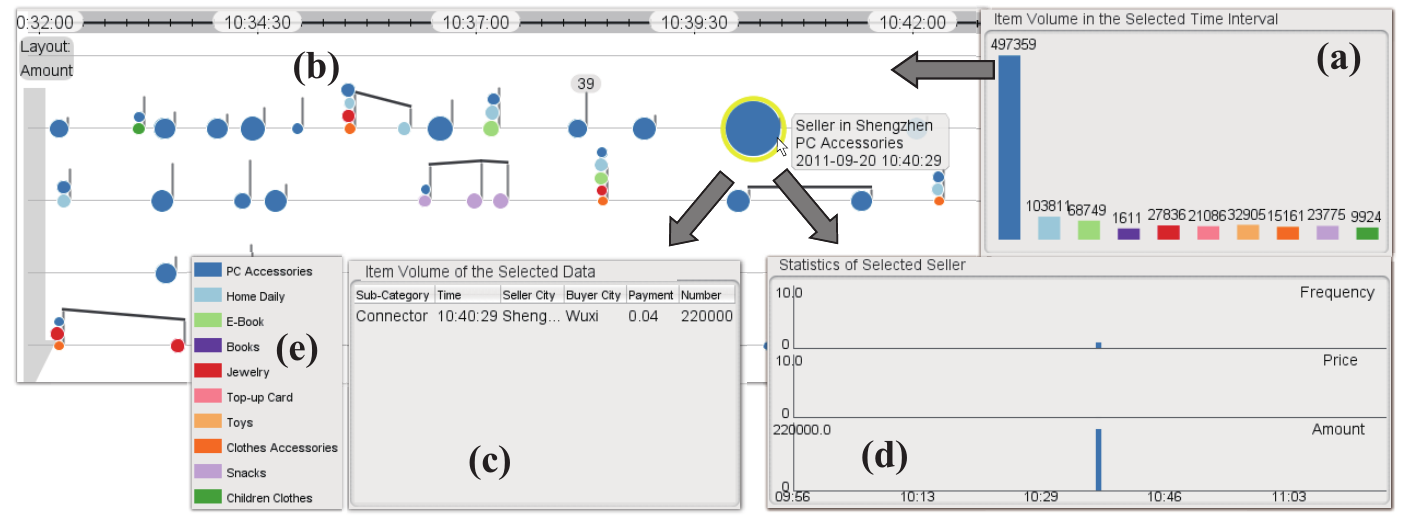
\includegraphics[width=\columnwidth]{KnotLines}
	\caption{KnotLine view from \cite{Xie:2014}. (a) Bar chart for the number of commodities in different categories. (b) The big knot indicates an unusually large number of commodities in a transaction. (c) Detailed information. (d) Statistical information. (e) Sales category legend.
	}
	\label{fig:knotlines}
\end{figure}

Similar to VAET \cite{Xie:2014}, Falcon was recently presented by Steed et al. \cite{steed:2017}.
Their system is focused on detecting correlative patterns in log and imagery data collected by 3D printers, which is highly irregular, includes missing values and has a high complexity in general.
Unlike the other systems, this visual analytics tool is designed from a manufacturing standpoint to discover defects and system performance issues or increasing production efficiency.
%The visualization of the system is based on the visual information seeking strategy.
Therefore, the system provides different line plots for each variable with individual level-of-detail control and filtering including an interactive statistical view (\autoref{fig:falcon}).
Consequently, multiple different variables can be displayed and examined by the analyst in order to find correlations (Q5) between those.
The system also provides a new visualization technique, called waterfall visualization, to combine overview and detailed view (Q1). 
This idea can be seen similar to the color charts by Ichikawa et al. \cite{ichikawa:2002}.
%Further, a comparative view is provided to analyze different variables of multiple configurations, which also includes pattern matching capabilities. 
%With the application of information scent, the system encodes quantitative values from similarity and statistical methods in the visualization in order to highlight relationships and reduce the search space. 
From an operational point of view, the system offers, similar to \cite{Xie:2014}, user driven analysis and helps to detect and highlight univariate and multivariate patterns from different angles.
%Technologically, the system is bin based, each bin contains a small subset of data points and the corresponding descriptive statistics. 
%Through the aggregation of bins, a higher level-of-detail abstraction can be achieved. 
%The above parts of the system can be applies well to other problem ares, however they also included visualizations specifically for the analysis of 3D printer data.
%One of those is a segmented time series view, which partitions a selected time series of a variable and also visualizes the images of the printing process next to it. 
Steed et al. were supporting a universal approach for Falcon to make it applicable in different domains. 
However, to support their specific analysis task, they included some non-generalizing functionalities. 
%By providing a reference time series, the system computes the similarity/dissimilarity of both series.
Similar to the model selection framework from Lu et al. \cite{Lu:2014}, they enable the analyst to compare the time series to a historical/user-defined time series. 
%Another feature specifically for 3D printers is the segmentation based on the build height as well as porosity detection.
%Whereas, these specific features provide important information for this use case, they make the system less generic and applicable to other areas. 
This comparison makes it easier to distinct between normal behavior and anomalies (Q6). 
As a consequence, the system grants analyst the ability for predictive maintenance, e.g. detecting a heat development pattern, which signals failure of the printer head in the near future. 
Currently the system does not support provenance information and the similarity/dissimilarity methods are limited to a single view.

\begin{figure}[htb]
	\centering
	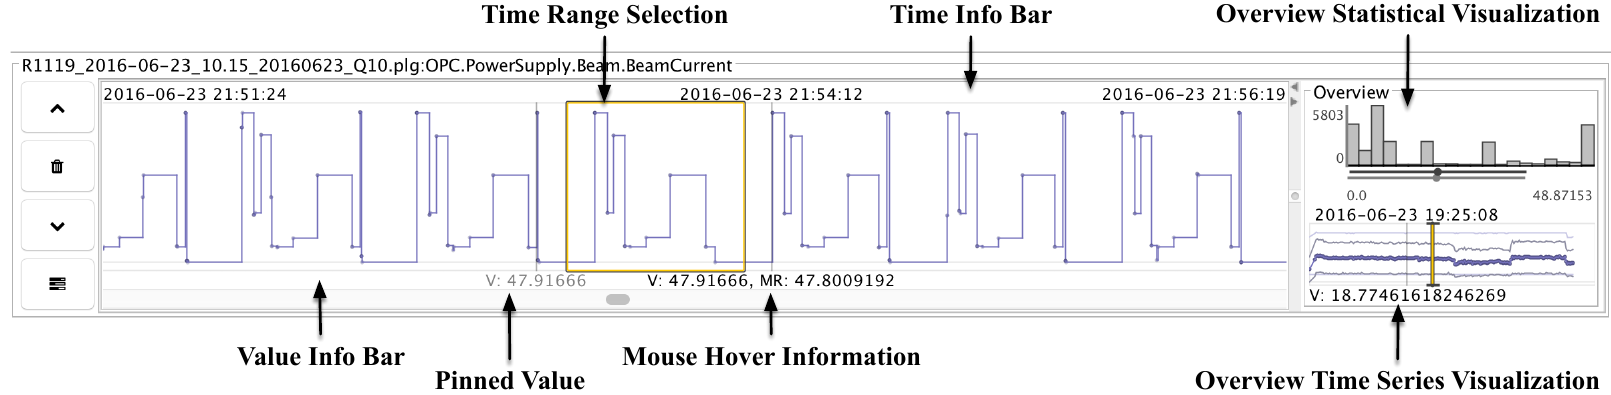
\includegraphics[width=\columnwidth]{Falcon}
	\caption{Time series visualization of one variable from \cite{steed:2017}
	}
	\label{fig:falcon}
\end{figure}

It has to be noted here, that unlike TimeSearcher \cite{Hochheiser:2004, buono:2005, buono:2007} or the peak preservation approach \cite{Hao:2012}, VAET \cite{Xie:2014} and Falcon \cite{steed:2017} do not incorporate a automatic prediction functionality.
They only assist analysts in examining time series, so that they can extract information about future behavior. 
Nevertheless, this allows them to provide better support to answer (Q4), (Q5), (Q6) and detect cause-effect relationships, which is typically not possible with other systems. 

Other application, which specifically focus on pattern detection can be found for patient treatment plans \cite{Gschwandtner:2011} or climate research \cite{Kehrer:2008}.
Whereas, the latter can also be interpreted as spatiotemporal as it detects regions in the atmosphere, which indicate climate change.
Similar to the focus of Hao et al. \cite{Hao:2009, Hao:2011}, Janetzko et al. \cite{janetzko:2014} focuses on power consumption in data centers, more specifically on anomaly detection of the corresponding time series.
In the same application context is the system of McLachlan et al. \cite{McLachlan:2008}. 
Similar to Falcon \cite{steed:2017}, this system is supporting large scale time series, in particular it was developed for large scale systems management of network devices.
Scalability is an issue, which all other systems are not able to handle properly.
Falcon \cite{steed:2017} is the only system in this survey to provide similar capacity, although in a different application area. 
These last system were just described shortly as they touch the topic of the survey only peripherally, but should provide the reader with a starting point for further research.

\subsection{Modeling\label{sec:modeling}}
%%The modeling steps builds upon the previous data preprocessing and feature selection process. 
%%This assumes the analyst already has an understanding about the data and prepared it for analysis.
%%Further, he took care of feature generation and feature selection in order to represent the data accordingly. 
%%During this step, systems support the analyst with e.g. subspace exploration, training set modification, parameter tuning. \cite{Lu:2017}\\
%An popular approach for general time series analysis is from Buono et al. \cite{buono:2005} and focuses explicitly on automatically finding similar patterns compared to a user specified pattern.
%The system was built upon TimeSearcher proposed by Hochheiser and Shneiderman \cite{Hochheiser:2004}, which concentrates on high usability even for users without specialized skills such as in statistics.
%%Based on their idea, Buono et al. continued with using timeboxes, i.e. rectangular regions that filter the data and reduce the scope of each search.
%%Their updated version adds another variant for pattern search in the remaining data. 
%%Further, they also allow users to work with long time series of multiple heterogeneous variables. 
%However, these two version of TimeSearcher are more interested in data exploration and consequently would be located either in the data preprocessing or as supporting tool in the feature engineering step. 
%%For data exploration the user is initially presented with a multivariable time series viewer, which allows to visually analyze multiple variables in parallel on different levels-of-detail.
%%In order to detect reoccurring and similar patterns, the user highlights a found pattern within the time series and the system uses a similarity-based search to find other occurrences. 
%%Therefor, the search space can be limited to only interesting areas.
%%The initial matches of the given pattern can afterwards be refined to support the analysis goal better. 
%%This process of returning many results and consequently enable the user to reduce the outcome to his/her liking, can also be found in spatiotemporal approaches (\autoref{sec:spatiotemp}), esp. in the template driven approach of \cite{malik:2014}.
%%Moreover, TimeSearcher also provides different data transformations to match patterns more easily. 
%%One drawback of the system is that it cannot deal with missing data points and pattern matching is very depended on the user's chosen parameters.
%For modeling the updated version of TimeSearcher by Buono et al. \cite{buono:2007} is of greater interest.  
%For its prediction, it resorts on the similarity-based approach, which was used in the previous version \cite{buono:2005} to detect time series with similar behavior.
%In order to provide the analyst with an better overall understanding of the selected subset of time series, the system offers a summarized view based on a river plot, which also incorporates confidence bands (bottom right of \autoref{fig:timesearcher}).
%The actual prediction is computed by extrapolating only those time series, which were identified as similar to the target time series.
%%As in \cite{buono:2005} the system is meant for users without statistical knowledge.
%In order enable the analyst to select a better model, the simultaneous preview interface allows to compare multiple parameter choices as well as different modeling techniques, such as smoothing, in parallel (\autoref{fig:timesearcher}). 
%Given the data-driven nature of the system, this requires the analyst to provide larger datasets compared to a model-driven approach.
%However, the simultaneous preview interface simplifies the modeling process and makes it accessible to untrained users and allows experienced analysts to get a better insight.
%
%\begin{figure}[htb]
%	\centering
%	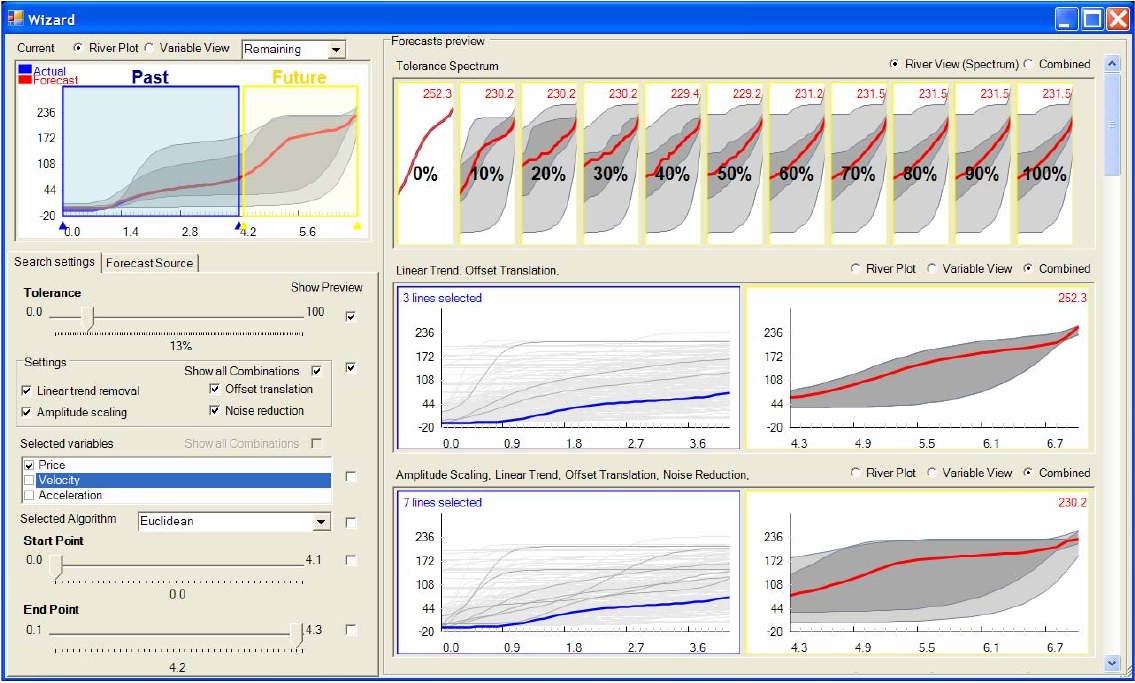
\includegraphics[width=\columnwidth]{TimeSearcher}
%	\caption{TimeSearcher's \cite{buono:2007} simultaneous preview interface
%	}
%	\label{fig:timesearcher}
%\end{figure}
%
%In practical scenarios the requirement to have large amounts of data points can often be a problem, which makes the systems \cite{Hochheiser:2004, buono:2005, buono:2007} less valuable.
%Consequently, a model-driven system, which requires less data points, is preferred.
%The approach of \cite{ichikawa:2002} could be seen as such system as it utilizes external simulations models.
%However, it is not supporting the modeling process and is therefore only seen as system for result exploration.
%On the other hand, TiMoVa a system, which explicitly provides model parameter selection was proposed from B{\"o}gel et al. \cite{boegl:2013}.
%The system is designed after the Box Jenkins method and is only supporting the model specification and selection process.
%For model specification, i.e. selection of an appropriate model type and its order, they provide autocorrelation function and partial autocorrelation function plots.
%These plots are also utilized by the analyst to select the model's parameters.
%A big drawback of the system are the assumptions about the preprocessed data. 
%It requires a time series without missing values and only supports univariate analysis.


\subsection{Result Exploration and Validation\label{sec:exploration}}
%Subsequent to the creation of the model, the analyst wants to explore the results/predictions and eventually compare the performance between several models. 
%Therefore, system are often highly interactive to provide the analyst as much freedom as possible.\cite{Lu:2017}\\
%An older Visual Analytics approaches is from Ichikawa et al. \cite{ichikawa:2002}.
%They wanted to enable analysts to predict multiple daytime stock prices and simultaneously visualize a set of predictions from different simulation systems. 
%This means, unlike other systems, their system only supports result exploration and/or model selection by efficiently visualizing a vast amount of predictions.
%As a consequence, the visualization includes multiple predictions for multiple stocks. 
%One major finding was, visualizing multivariate predictions in a 3-dimensional space creates high levels of occlusion, thus, it is not suitable.
%Instead, the system utilizes line charts with cluttering control and color charts with level-of-detail control. 
%%The line charts support multivariate scaling, i.e. the time axis can be scaled differently to focus on certain areas, e.g. areas with higher discrepancies of the simulations.
%%Further, the lines are colored differently, depending on the amount of overlap/uniform predictions.
%The color chart tries to reduce the complexity of all simulations by clustering similar predictions and reducing the time series to its key elements, i.e. the overall trends of each cluster.
%This allows the analyst to detect discrepancies between the clusters.
%Further, he is able to compare specific predictions with the overall trend. 
%%The color chart is composed of horizontal color-bands for each prediction, whereas a vertical color band can be seen as a period in time. 
%%In order to improve the visualization, the different color-bands are cluster based on the user-specified level-of detail. 
%%This results in a smaller amount of horizontal color-bands where the individual properties are diminished. 
%%In the workspace the above plots can be displayed with different axis.
%For additional comparison, the systems workspace visualizes a set of predictions for different parameter ranges (e.g. sales organizations) as well as different stocks.
%Consequently, the user can detect trends concerning the whole stock market.  
%However, due to the amount of simulations displayed, it can be hard to extract specific information.
%
%During the evaluation of TiMoVa \cite{boegl:2013}, they found that an actual prediction functionality would provide additional value for the analyst.
%Therefor, they included a result exploration and validation functionality.
%This allows the analyst to adjust different model parameters and see the changes in the corresponding prediction visualizations, which gives him feedback about the adequateness about the chosen model. 
%Similar to \cite{buono:2007}, the prediction is incorporated with confidence bands to express the models certainty. 
%Additionally, they specifically visualize the difference of true and predicted values for each data point as well as the direction (positive or negative).
%This gives the analyst a quick overview if the model is constantly over- or underestimating the time series as well as how long and often this occurs.

%One goal in time series analysis is detecting patterns.
%These patterns help analysts to better understand their data and enables them to formulate improved hypotheses for future developments. 
%Further, they allow analysts to detect unusual occurrences, which makes it possible to spot undesired behaviors in advance and react accordingly. 
%Such anomalies can include fraud attempts, higher server loads or bad configurations of manufacturing machines.\\

%However, in a practical environment it is often necessary to evaluate multiple time series in parallel or deal with multidimensional input variables.
%In order to solve these problems, visual analytics approaches for simple time series are not sufficient anymore.\\ 

%\subection{Data Correlations}

%A more specialized data-driven visual analytics approach was proposed from Xie et al. \cite{Xie:2014}.
%The difference to other approaches can be found in the application area of customer-to-customer e-transaction time series. 
%The time series consists of transactions between the a seller and a buyer.
%However, the commodities as well as the buyer can vary greatly.
%Finding patterns in such time series helps analysts to understand temporal and contextual connections between multiple transactions of one seller, e.g. high number of transactions with same seller/ with same commodity.
%This can be extended to gain an understanding of the overall selling process or identifying fake transactions.
%For analysis the system employs a iterative process consisting of two main visual analytics components, an overview component and a detail component.
%The overview component proposes possible salient transactions. 
%Therefor, a decision tree learner calculates a saliency score for each transaction and a certain analysis task.
%This learner addresses basic features (e.g. commodity, order amount), textual features (e.g. sensitive words in comments) and temporal features (e.g. transaction amount of seller within on time period).
%The latter is difficult to address by a decision tree, hence the systems harnesses the transaction frequency of a seller in a user defined time interval.
%Consequently, the saliency scores are displayed in a time-of-saliency map with an user adjustable level-of-detail. 
%The detailed view is used to gain more insight on specific transactions, which were selected by the user in the overview.
%For visualization, they introduce a musical notation inspired visual metaphor, called KnotLines (\autoref{fig:knotlines}).
%The amount of transactions in one section (e.g. books) defines the size of the corresponding note head, where missing values are explicitly marked to catch the attention of an analyst.
%For each time interval the sections' heads are placed on the same note stem, where the length represents the total payment per seller and per time interval.  
%In order to capture the relationship over multiple time intervals, the stems of one seller are connected by beams.
%This view enables the analyst to observe multiple attributes as well as temporal and contextual correlations of transactions and find salient transactions.
%The identified salient transactions are fed back to decision tree learner, which changes the predictions of the unknown transactions.
%A big drawback of the initial computation of saliency values is the need for training data. 
%Analysts are required to annotate features of training transactions, unlike most other approaches introduced in this survey, which do not require this additional step. 

%\begin{figure}[htb]
% \centering
% 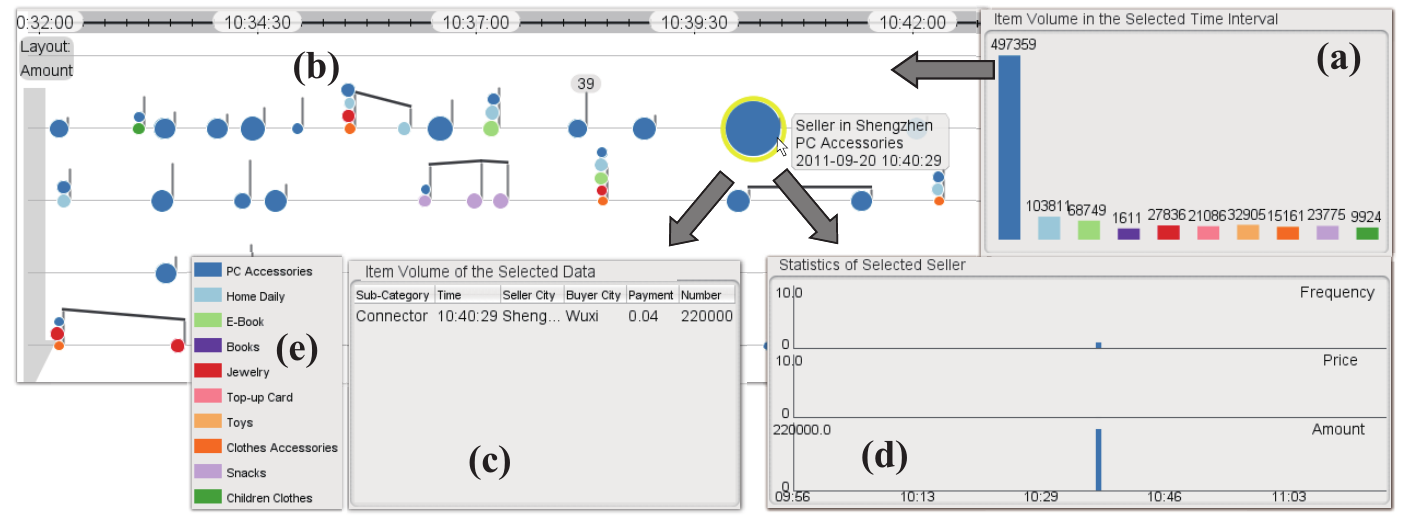
\includegraphics[width=\columnwidth]{KnotLines}
% \caption{KnotLine view from \cite{Xie:2014}. (a) Bar chart for the number of commodities in different categories. (b) The big knot indicates an unusually large number of commodities in a transaction. (c) Detailed information. (d) Statistical information. (e) Sales category legend.
% 	}
% \label{fig:knotlines}
%\end{figure}
%
%Similar to \cite{Xie:2014}, another specialized system was recently presented by Steed et al. \cite{steed:2017}.
%Their approach is focused on understanding patterns in log and imagery data collected by 3D printers, which is highly irregular, includes missing values and has a high complexity in general.
%Unlike the other systems, this visual analytics tool is designed from an manufacturing standpoint to discover patterns related to defects and system performance issues, optimizations to avoid defects and increasing production efficiency.
%The visualization of the system is based on the visual information seeking strategy.
%Therefor, the system provides different charts for each variable with individual level-of-detail control and filtering including an interactive statistical view (\autoref{fig:falcon}). 
%They also provide a new visualization technique, called waterfall visualization, to combine overview and detailed view, which is similar to the idea of color charts by \cite{ichikawa:2002}
%Further, a comparative view is provided to analyze different variables of multiple configurations, which also includes pattern matching capabilities. 
%With the application of information scent, the system encodes quantitative values from similarity and statistical methods in the visualization in order to highlight relationships and reduce the search space. 
%From an operational point of view, the system offers, similar to \cite{Xie:2014}, user driven analysis and helps to detect and highlight univariate and multivariate patterns from different angles.
%Technologically, the system is bin based, each bin contains a small subset of data points and the corresponding descriptive statistics. 
%Through the aggregation of bins, a higher level-of-detail abstraction can be achieved. 
%The above parts of the system can be applies well to other problem ares, however they also included visualizations specifically for the analysis of 3D printer data.
%One of those is a segmented time series view, which partitions a selected time series of a variable and also visualizes the images of the printing process next to it. 
%By providing a reference time series, the system computes the similarity/dissimilarity of both series.
%Another feature specifically for 3D printers is the segmentation based on the build height as well as porosity detection.
%Whereas, these specific features provide important information for this use case, they make the system less generic and applicable to other areas. 
%Further, the system currently does not support provenance information and the similarity/dissimilarity methods are limited to the segmented time series view.

%\begin{figure}[htb]
%	\centering
%	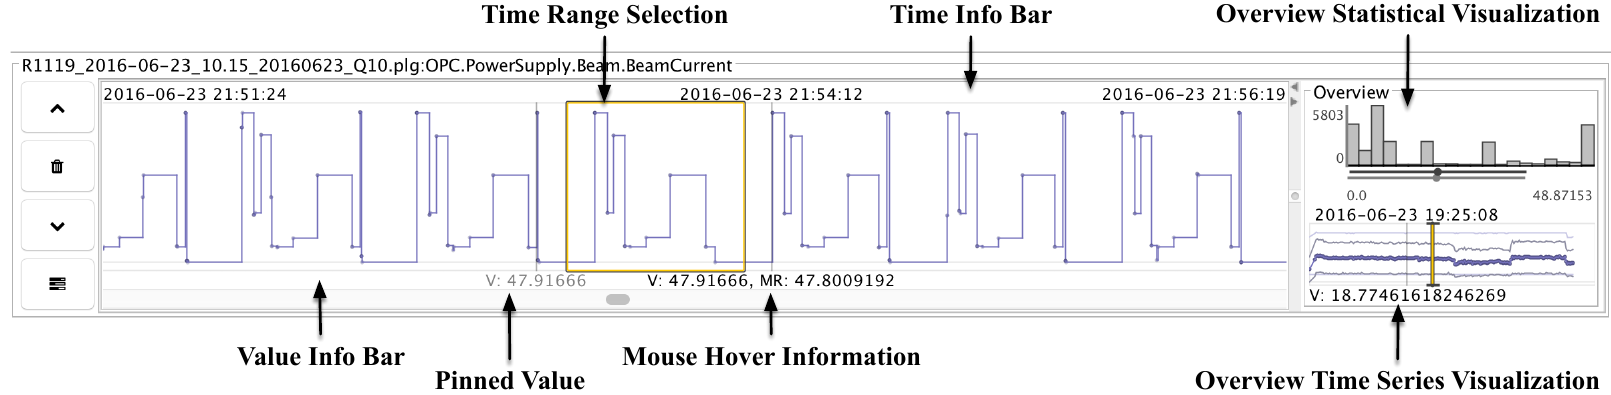
\includegraphics[width=\columnwidth]{Falcon}
%	\caption{Time series visualization of one variable from \cite{steed:2017}
%	}
%	\label{fig:falcon}
%\end{figure}
%
%Other application specific approaches involve pattern detection within patient treatment plans \cite{Gschwandtner:2011} or hypothesis generation for climate research \cite{Kehrer:2008}.
%Whereas, the latter can also be seen as spatiotemporal as it tries to detect regions in the atmosphere, which indicate climate change.
%Similar to \cite{Xie:2014}, Janetzko et al. \cite{janetzko:2014} focuses specifically on anomaly detection.
%However, the underlying time series is based on server power consumption.
%In the same application context is the system of McLachlan et al. \cite{McLachlan:2008}. 
%Their analytics tool was developed for system management and is also viable for large time series, i.e. hundreds of parameters across thousands of network devices.
%Other multivariate systems, such as \cite{ichikawa:2002, buono:2005, buono:2007}, are often not able to present these amounts clearly.
%The application of \cite{steed:2017} is one of the few to provide similar capacity, although a different application area. 
%%\subsection{Peak Preservation \label{subsec:peak}}
%Time series prediction with peak preservation poses a similar problem as pattern and anomaly detection. 
%%However, preserving peaks for prediction can be seen as an additional step. 
%The identified patterns/peaks need to be included in the systems forecast.
%%The application areas for such systems is also differing from trend based predictions, which try to smooth and generalize to have a more consistent prediction. 
%%However, for example when analyzing power consumption time series in data centers, it is important to preserve peaks and their patterns.
%An systems which also includes this additional step in the prediction process is from Hao et al.\cite{Hao:2011, Hao:2009}.
%They applied an automated peak preserving smoothing method in order to reduce noise and get a more reliable prediction as well as retain the seasonality of the data.
%Thereby, the analyst is able to determine the influence of more recent measurements, i.e. how far back in time seasonality is considered in the smoothing process. 
%Otherwise, the system is comparable to \cite{buono:2007}.
%This idea is inherited in \cite{Hao:2012}, where the peak preservation is combined with an automated motif/pattern detection, which includes detecting overlapping patterns. 
%Similar to \cite{buono:2007}, depending on the user's preference, the detected patterns can be aggregated to increase their significance.

\section{Spatial Time Series\label{sec:spatiotemp}}
The previous section presented an overview of systems for abstract time series analysis. 
However, for other application areas, such as crime prevention as well as emergency and epidemic intelligence, not only the temporal information is valuable, but also the spatial information.
Typically, spatial information has a hierarchical categorization structure, which can be filtered.
Further, the data categories are processed either as aggregated time series over a spatial location (e.g. county, zip code, collection station) or represent a spatial snapshot of a small time aggregate (e.g., day, week).
Andrienko et al. \cite{Andrienko:2008, Andrienko:2010:Space} also found that geospatial analysis has a higher complexity and automated methods cannot adequately solve this task. 
It requires the domain knowledge of a human analyst in order to solve these problems comprehensively.
However, as a result of the high dimensionality of data, an analyst needs support from visual analytics systems.\\

An approach, which can be seen between temporal and spatiotemporal is from Andrienko et al. \cite{Andrienko:2010}. 
They include spatial dimensions, but their analysis is largely based on abstract time series compared to the following approaches.
Similar to the peak preserving approach from Hao et al. \cite{Hao:2009,Hao:2011,Hao:2012}, they ensure local specialties are represented in the prediction. 

Maciejewski et al. \cite{maciejewski:2011} are proceeding from their previous work \cite{maciejewski:2008, maciejewski:2007} and focus on categorical medical event data.
Events consist out of locations in time and/or space, whereas each event can be placed into a hierarchical categorization structure.
%Specifically, they used a data set for detecting adverse health events using pre-diagnosis information from emergency departments.
Similar to TimeSearcher \cite{Hochheiser:2004, buono:2005, buono:2007}, TiMoVa \cite{boegl:2014, boegl:2013} and peak preservation \cite{Hao:2009, Hao:2011, Hao:2012} confidence bands are established in order to answer (Q7).
%The system itself provides a line chart with certainty bands and a colored 
A Geospatial view gives an overview of the percentage of events in a certain area, e.g. patients at an emergency department, which where classified with respiratory syndromes (\autoref{fig:hotspot}).
%Further, the user is able to apply filtering on a fine and coarse-grained level. 
One important part is, the systems differentiates between the time series and the geospatial prediction.
%The time series prediction is achieved by cumulative summation or a Seasonal Trend decomposition based on locally weighted regression.
For multivariate time series data, each event category is modeled as a separate time series signal and consequently forecast. 
%Equivalent to the time series prediction, the granularity/level of aggregation (e.g. state, county, etc.) for geospatial predictions can be adjusted by the user.
For geospatial predictions, the system utilizes density estimation to determine the spatial distribution of the time series prediction. 
%utilizes a kernel density estimation, which allows to display the spatiotemporal distribution on a fine-grained level.
In order to predict anomalies, e.g. outbreaks of diseases, the system calculates the difference between the predicted and the actual values and highlights areas above a user specified threshold (yellow diamonds in \autoref{fig:hotspot}).

\begin{figure}[htb]
	\centering
	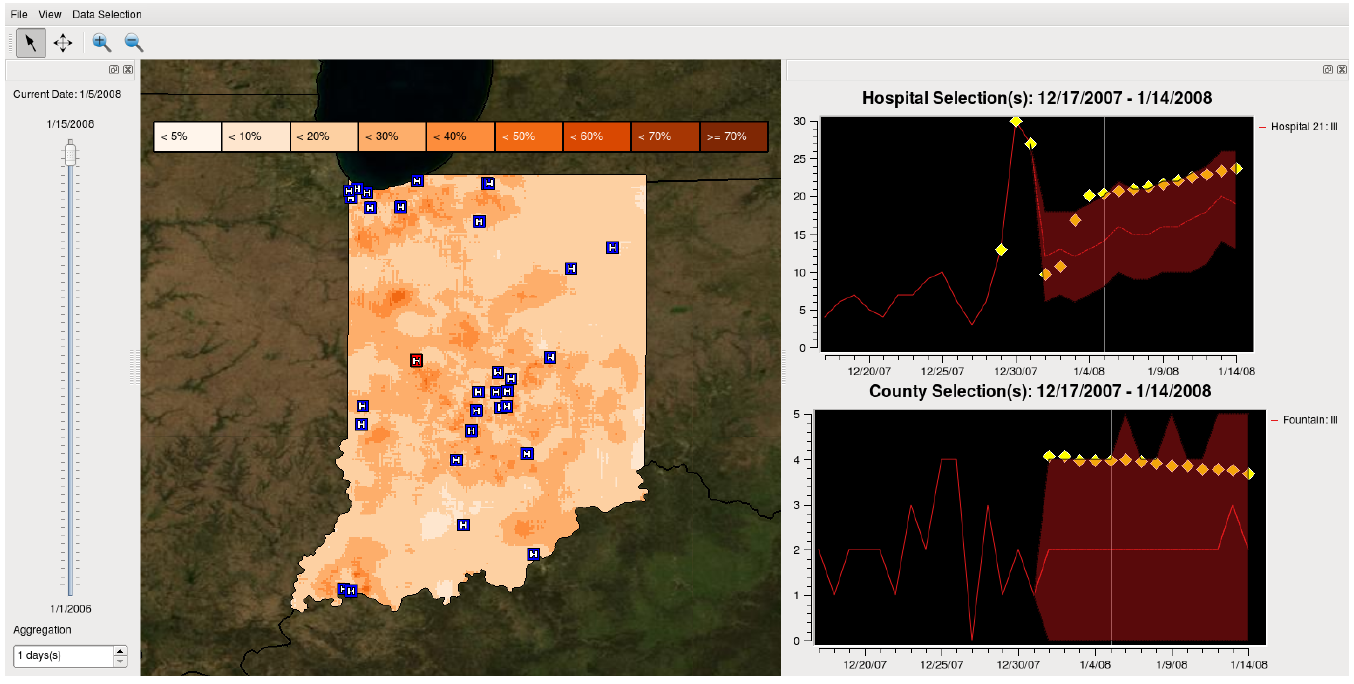
\includegraphics[width=\columnwidth]{Hotspot}
	\caption{Interactive visual analytics environment from \cite{maciejewski:2011}. Analysis of respiratory syndrome counts in Indiana on county level. The yellow diamonds indicate temporal alerts, the white line the current day and the transparent polygon the prediction's confidence.
	}
	\label{fig:hotspot}
\end{figure}

Another system also from Maciejewski et al. \cite{maciejewski:2010} follows a similar approach.
They target multivariate data with high signal to noise ratio and a degree of uncertainty.
Equivalent to \cite{maciejewski:2011} the system provides a linked environment of geospatial data and time series graphs and separates time series and spatial forecast.
%allows users to filter data.
%Additionally, the system also uses cumulated summation and Kernel Density Estimation. 
The major difference is, this work focuses on finding and understanding patterns, rather than only predicting them.
Therefore, the system establishes temporal contour maps, which are overlaid contour maps over a period of time. 
This allows the analyst to view shifting hotspots across time and analyze the movements of trends and patterns over this period.
Further, the system allows to search for correlations between multiple variables via overlaying contour maps, heat maps and/or including height. 
However, one issue with this visualization is, it only works in a three dimensional variable space and cannot help to find correlations in a higher dimensional space. 
Moreover, in both systems aggregating too many data points, may yield to largely exaggerated hotspots or a uniform surface, as a result of too many hotspots. 

Recent work from Malik et al. \cite{malik:2014} focuses, comparable to TimeSearcher \cite{Hochheiser:2004, buono:2007, buono:2005, Xie:2014} and the model selection framework \cite{lu:2014}, on a visual analytics approach that provides non statistic experts a proactive and predictive environment, which allows them to utilize their domain expertise.
Analogous to Maciejewski et al. \cite{maciejewski:2011, maciejewski:2010}, the systems is using the same approach in order to predict time and space.
%the system applies seasonal trend decomposition based on locally weighted regression and Kernel Density Estimation for its predictions.
One issue which was identified by Malik et al. in Maciejewski \cite{maciejewski:2011} earlier work was that domain experts need additional guidance in order to improve their analysis.
This motivation is equivalent to the idea behind TimeSearcher \cite{Hochheiser:2004, buono:2007, buono:2005} by providing the preview interface or the baseline models from the model selection framework \cite{lu:2014}.
Geospatial and temporal scale templates present the analyst with a starting point and avoids searching through the complete parameter space.
%For the geospatial templates, the system separates the space in subregions and filters for regions, which show a high predicted activity and provide sufficient data. 
Further, the system allows the user to interactively change the initial templates to include e.g. police beats.
%and avoid zero counts with no predictive statistical value.
In order to compensate for insufficient data points, the system can make use of demographically similar neighborhoods within a certain radius around that area. 
Temporal templates follow the idea of peak preservation, such as in the work of Hao et al. \cite{Hao:2009, Hao:2011, Hao:2012}.
%Trends can occur on different scales of time. 
%Therefore, the system provides a clock view to highlight high activity on a hourly granularity.
An additional improvement to the previous systems includes the easier access to observe trends on different scales of time, i.e. on hourly, daily and monthly basis.

In contrast to all the previous spatiotemporal approaches Andrienko et al. \cite{Andrienko:2010:Space} did not use the same prediction approach, but applied self-organizing maps (\textit{SOM}) for either spatial or temporal prediction.
% Seasonal Trend decomposition and kernel density estimation, but applied self-organizing maps (\textit{SOM}) for spatial and temporal prediction.
SOMs can be seen as a combination of clustering and dimensionality reduction based on the similarity of space and time, therefore this can be seen at least alike to the similarity-based approach of TimeSearcher \cite{Hochheiser:2004, buono:2007, buono:2005}.
The SOM method is applied to spatial situations that occur in different time units and to local temporal variations that occur in different places.
This idea can also be found in earlier work from Andrienko \& Andrienko \cite{Andrienko:2005}.
The more recent approach is applying feature images and index images (\autoref{fig:som} top and bottom of each cell) for the spatial and temporal dimension.
%Feature images do not represent detailed information, they solely display the relative magnitude of the attribute, i.e. different attributes can have different scales, therefore they cannot be used for attribute comparison and only give an overview.
%The implementation is done by either maps and multi-attribute mosaics for spatial data or temporal mosaics for temporal data (\autoref{fig:som} left and right).
Feature images are used in order to analyze the magnitude of attributes.
Spatial data is represented as map, whereas temporal data as temporal mosaic, which has a large correspondence to the color charts of Ichikawa et al. \cite{ichikawa:2002} and the waterfall visualization of Falcon \cite{steed:2017}.
Index images show either the temporal or spatial elements, which provide the data source for one SOM matrix cell, depending on the analysis context.
%More precisely, a black cell or territory compartment is contributing to the visualization of the above feature image.  
In order to enable the analyst to find correlations between time and space, multiple SOM cells with different feature images and index images are displayed in a matrix.
%Additionally, an aggregative view provides an overview of space or time.
Additionally, a second visualization aggregates the index images to display the respective other dimension.
This allows the analyst to determine at which time a certain spatial cell is present or at which location a certain temporal cell occurs.
The temporal aggregation shows again a similar structure as the color charts of Ichikawa et al. \cite{ichikawa:2002} and the waterfall visualization of Falcon \cite{steed:2017}.
The evaluation of the system shows that it is applicable for detecting expected as well as unexpected results.
This allows analysts to either find evidence, which supports their previous formed hypothesis or discover new connections, which enables them to make assumptions about future events. 

\begin{figure}[htb]
	\centering
	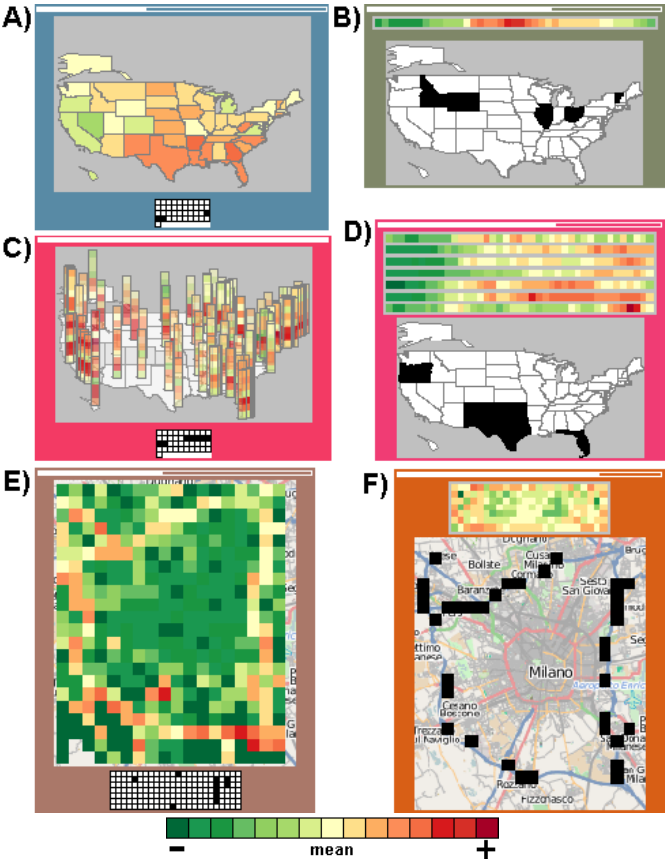
\includegraphics[width=\columnwidth]{SOM}
	\caption{SOM approach from \cite{Andrienko:2010:Space}
		Left column: grouping of spatial situations.
		Right: grouping of places according to temporal variations of attribute values.
		A,B: single attribute. 
		C,D: multivariate data with 7 attributes. 
		E,F: one attribute with higher temporal and spatial detail. 
		The	upper image in each cell is the feature image, the lower im-
		age is the index image.
	}
	\label{fig:som}
\end{figure}

%Coming back to the first approaches utilizing seasonal trend decomposition.
Aside from medical and crime data sets, spatiotemporal data can also be helpful in other domains. 
Similar to the first approaches, seasonal trend decomposition can be used in context of social media anomaly detection \cite{Chae:2012, Thom:2012}. 
This can help to increase situational awareness of local events as well as provide insight for investigations and incidents, their severity and consequences.


% TODO Useless stuff
%One of the first visual analytics approaches to spatiotemporal time series prediction is from Yue et al. \cite{yue:2009}.
%They proposed a blackboard approach, which mainly focuses on supporting terrorism investigations.
%The system is split in two parts, one for predicting missing information, e.g. terrorist group name, and another for predicting future events based on a time series. 
%Due to the topic of this survey, the following only focues on the second part.
%One important aspect of the system is the work with heterogeneous knowledge sources (e.g. Autoregression model, Moving Average model), which contain the necessary domain knowledge to solve a problem.
%A second key component is the AI blackboard, which is used as interaction with the user. 
%The importance originates from the fact that the system is meant to interactively support the user in predicting missing information by providing proposals and taking feedback from the analyst.
%%Due to the application area, the systems determines the best knowledge sources to perform predictive analysis (e.g. on the number of terrorism occurrences) based on resources constraints (e.g. deadline).
%%The analysis itself is a three steps process including a data classification based on the selected knowledge sources, followed by visualizing these on a map and temporal view.
%%In the last two stages, the analyst is able to gain more insight and can adjust the confidence of the possible solutions as needed.  
%%The final result is a confidence weighted aggregation over all three stages including the corresponding user feedback. 

\section{Summary}
%As a result of this survey I found 
For time series prediction we can separate two major directions: temporal time series and spatiotemporal.
Temporal time series analysis mainly follows data-driven interactive approaches, which include the user in the pattern finding process by providing supportive features such as the simultaneous preview interface \cite{buono:2007}, the segmented time series view \cite{steed:2017} or the KnotLines \cite{Xie:2014}.
They are all enabling the analyst to better understand the data, generate hypothesis and predict future developments or anomaly occurances.
Spatiotemporal time series add another important dimension, which makes automated analysis more complicated. 
Visual analytics systems approach this problem, unlike exclusive temporal time series, often with a model-driven approach. 
Further, the systems have to enable the user to select spatial and temporal resolution.
The system of \cite{malik:2014} even suggests different templates to makes the systems more accessible to domain experts.\\
One important drawback all systems, besides \cite{steed:2017,McLachlan:2008}, have is often the missing scalability to large amount of parameters and different time series at once. 
Although, this can be seen as common problem for multi-product companies, customer-to-customer online platforms, etc.
On the other hand the current visual analytics system offer a broad range of application areas including manufacturing, medical, environmental and social media oriented. 

%\bibliographystyle{abbrv}
%\bibliographystyle{abbrv-doi}
%\bibliographystyle{abbrv-doi-narrow}
\bibliographystyle{abbrv-doi-hyperref}
%\bibliographystyle{abbrv-doi-hyperref-narrow}

\bibliography{bibliography}
\end{document}
